\documentclass{article}

% Language setting
% Replace `english' with e.g. `spanish' to change the document language
\usepackage[english]{babel}

% Set page size and margins
% Replace `letterpaper' with `a4paper' for UK/EU standard size
\usepackage[letterpaper,top=2cm,bottom=2cm,left=3cm,right=3cm,marginparwidth=1.75cm]{geometry}

% Useful packages
\usepackage{amsmath}
\usepackage{graphicx}
\usepackage[colorlinks=true, allcolors=blue]{hyperref}
\usepackage{tabularx,booktabs}
\newcolumntype{Y}{>{\raggedright\arraybackslash}X}

\title{From Accuracy to Adoption: Explainability and Reporting Standards in Medical Imaging AI}
\author{Alan Weng, Nipun Deelaka Pathirage, Neha Keshan}

\begin{document}
\maketitle

\begin{abstract}
Artificial intelligence (AI) has achieved strong results in medical imaging tasks such as segmentation, detection, and classification. However, clinical adoption remains limited, with trust and reporting standards emerging as significant barriers. This review examines literature from 2020 to 2025 to evaluate the uptake of reporting guidelines and to assess how explainability and trust principles are addressed. Citation analysis of PubMed-indexed papers shows that fewer than 11\% referenced these frameworks within the last 10 years, with older standards like TRIPOD (2015) and CLAIM (2020) contributing a significant portion of citations. Furthermore, citation analysis within the last 5 years reveals that fewer than 7\% of papers referenced or used these frameworks. Barriers include low awareness, weak enforcement, and the complexity of newer checklists. Combining these results with qualitative findings, this review highlights the need for transparent reporting and stronger policy enforcement to support compliance. Achieving this requires standardized practices that enable trustworthy and effective AI integration in clinical workflows.


Resource website: \hyperlink{https://github.com/wengalan888/paper000}{https://github.com/wengalan888/paper000}


Keywords: medical imaging, artificial intelligence, explainable AI, reporting guidelines

\end{abstract}

\section{Introduction}
Medical imaging plays a vital role in modern healthcare by enabling the visualization of internal anatomy and pathology. Recent advances in artificial intelligence (AI) have introduced powerful tools for automating and enhancing the analysis of medical images. Review papers have documented significant advances in algorithms and clinical applications \cite{panayides_2020_ai,tang_2019_the,zakaria_2024_advancements}. Despite technical breakthroughs and high performance in controlled studies, the clinical adoption of AI models remains limited. 

Advancements in controlled studies have outpaced the rate of deployment, creating a gap between research and clinical application. Across multiple reviews and primary studies, several key factors have been identified as barriers to implementation including limited explainability, poor integration into clinical workflows, and a lack of standardized practices. One neglected barrier to further advancement is the low adherence to standardized reporting guidelines - such as CLAIM (2024), TRIPOD-AI (2024), DECIDE-AI (2022), and FUTURE-AI (2025) – designed to promote reproducibility and trustworthy AI for medical imaging. Research papers and clinical labs rarely utilize these guidelines, designed to establish trust and reliability in AI, which raises concerns about the transparency and dependability of the findings and claims.

To address these gaps, this review analyzes medical imaging AI literature from 2020 to 2025 to identify significant deployment barriers; to evaluate the adoption and usage trends of key reporting guidelines; and to explore emerging solutions–such as explainable and trustworthy AI frameworks–that may help align research results with clinical needs.

\section{Methods and Data}
\subsection{Literature Processing and Analysis}
Iterative searches were conducted with keywords such as "AI in medical imaging", "XAI", "deployment challenges," "trust in AI", and "adherence to medical imaging guidelines" on Google Scholar (multifaceted source encompassing PubMed, arXiv, IEEE publications). Publications released from 2020 to 2025 were specifically chosen in order to create a sample of approximately 30 to 40 works, including surveys, reviews, and primary studies.

A preliminary set of representative papers was used to co-develop a structured rubric (with generative AI assistance), including the following categories:

\begin{itemize}
\item Title, Year, Link, Type of Paper
\item Study Question, Hypothesis, Key Findings, Key Data
\item AI/ML Method, Imaging Task / Modality
\item Deployment Stage and Validation Context
\item Trust/Explainability Content
\item Limitations and Significance
\end{itemize}

For each paper, generative AI was used to generate initial summaries across the rubric fields. A subset of these outputs was then manually reviewed and validated for accuracy. This approach facilitated the synthesis of trends and the identification of gaps in guideline adoption.


\subsection{Citation Analysis of Reporting Guidelines}
The literature and guideline reviews were compiled into a list of more than 20 guidelines (e.g., CLAIM, TRIPOD‑AI, DECIDE‑AI, FUTURE‑AI) \cite{kolbinger_2024_reporting}. For each guideline, the citation count and the number of citations appearing in review/systematic review papers were collected from PubMed.

Using PubMed citation tools, the following were evaluated:

\begin{itemize}
\item The percentage of AI imaging papers (2015–2025 and 2020–2025) that cite any guideline
\item Trends in guideline citation
\item Disparities between older, widely cited guidelines and newer, underutilized ones
\end{itemize}

To validate these quantitative findings, two external studies documenting low CLAIM adherence in radiology AI literature were referenced \cite{belue_2023_the,burakkoak_2025_adherence}.

\section{Background and Literature Overview}
\subsection{Medical Imaging and AI Tasks}
Medical imaging employs various techniques to visualize the human body's anatomy and functions. Common ones include:

\begin{itemize}
\item X-ray and CT: Structural imaging using electromagnetic (ionizing) radiation.
\item MRI: Soft-tissue imaging using magnetic fields and radio waves
\item Ultrasound: Radiation-free imaging based on high-frequency sound wave reflections
\end{itemize}

While the methods of obtaining images vary across techniques, a standard clinical workflow involves image capturing, post-processing, interpretation of imaging, and diagnostic decision-making (refer to \cite{panayides_2020_ai} for a more comprehensive overview of these imaging tasks and AI's application in medical imaging).

Artificial intelligence (AI), more specifically, machine learning (ML) and deep learning (DL) are being employed to automate and enhance tasks such as:

\begin{itemize}
\item Segmentation: outlining anatomical or pathological regions
\item Detection: identifying abnormalities like tumors or fractures
\item Classification: predicting disease presence or type
\item Reconstruction: generating higher-quality images
\item Enhancement: enhancing image clarity or resolution
\end{itemize}

\subsection{Model–Task Taxonomy of AI in Medical Imaging}
Table 1 presents a task-to-model taxonomy, mapping common neural architectures (e.g., U-Net, CNNs, transformers) alongside representative performance metrics extracted from reviewed literature, showing the performance benefits AI brings across clinical domains. 


\renewcommand{\arraystretch}{1.5} % Increase vertical spacing more

\begin{table}[htbp]
\caption{Model--Task Taxonomy for AI in Medical Imaging}
\label{tab:model-task-taxonomy}
\normalsize % bigger text than footnotesize
\begin{tabularx}{\textwidth}{@{}p{2.4cm} p{3.2cm} Y Y Y@{}}
\toprule
\textbf{Task} & \textbf{Models / Algorithms} & \textbf{Example Papers \& Years} & \textbf{Key Datasets} & \textbf{Metrics (Source)} \\
\midrule
Segmentation &
U-Net, nnU-Net, TransUNet, SAM &
Clinical Applications Review \cite{obuchowicz_2024_clinical}; Seg. TAI Review \cite{teng_2024_a}; DL MRI Cardiac \cite{bernard_2018_deep}&
TCIA brain metastases \cite{obuchowicz_2024_clinical}; ACDC cardiac MRI; MoNuSAC nuclei \cite{teng_2024_a}&
Dice $\ge$0.90 (ACDC cardiac MRI) \cite{bernard_2018_deep}; Sens. 89\% (brain metastases) \cite{obuchowicz_2024_clinical} \\[0.5em]

Detection &
Faster R-CNN, YOLOv8, RetinaNet, 3D ResNet, Swin Transformer &
Emerging Trends \cite{oyeniyi_2024_emerging}; COVID-19 CT DA \cite{kollias_2024_domain}; JRC Innov. \cite{comtev_2025_aidriven} &
COV19-CT-DB \cite{kollias_2024_domain}; LUNA16 lung nodules \cite{comtev_2025_aidriven}; LIDC-IDRI \cite{oyeniyi_2024_emerging} &
Sens. 94.7\% (LUNA16) \cite{comtev_2025_aidriven} \\[0.5em]

Classification &
ResNet, DenseNet121, ViT, DCNNs &
Diag. Imaging Rev \cite{khalifa_2024_ai}; Breast Cancer Rev \cite{zheng_2023_overview}; Glaucoma Rev \cite{paulo_2024_advancements} &
TCGA/TCIA multi-modal \cite{tang_2019_the}; REFUGE fundus \cite{paulo_2024_advancements}; Breast MRI \cite{zheng_2023_overview}&
Acc. 99.1\% (breast cancer) \cite{zheng_2023_overview}; Acc. 92\% (prostate cancer) \cite{obuchowicz_2024_clinical} \\[0.5em]

Reconstruction &
GANs (CycleGAN, UnetGAN), nnU-Net denoising, DLIR, AutoML-GAN &
Informatics Rev \cite{panayides_2020_ai}; MDPI Workflow Rev \cite{obuchowicz_2024_clinical} &
CT low-dose \cite{obuchowicz_2024_clinical}; MRI motion artifacts \cite{panayides_2020_ai} &
SNR (up 54\% grey matter; 60\% white matter; DLIR) and CNR (up 58\% BGA; up 50\% PCF; DLIR) \cite{obuchowicz_2024_clinical}; \\[0.5em]

Enhancement &
Prob. U-Net, SRCNN, nnU-Net variants &
Radiogenomics Inf. \cite{panayides_2020_ai}; Infrared Breast XAI \cite{raghavan_2024_explainable}; AI-Driven Innov. \cite{comtev_2025_aidriven} &
UK Biobank MRI \cite{panayides_2020_ai}; DMR-IR thermal breast \cite{raghavan_2024_explainable}&
Dice = 0.96 (respiratory motion prediction) \cite{obuchowicz_2024_clinical}; Improved tumor boundary clarity (thermal breast) \cite{raghavan_2024_explainable} \\[0.5em]

Report Generation &
VLMs (GPT-4V, Gemini), Transformer+OPT, RAG &
Multimodal GenAI \cite{rao_2025_multimodal}; Radiograph Reporting \cite{huang_2025_efficiency} &
MIMIC-CXR \cite{rao_2025_multimodal}; Institutional radiograph corpus &
15.5\% time saved/report \cite{huang_2025_efficiency}; Accuracy parity (GPT-4V) \cite{rao_2025_multimodal} \\

\bottomrule
\end{tabularx}
\end{table}

\subsection{Literature Review: Trust and Adoption in AI for Medical Imaging}
Several in-depth reviews covered the technical advancement of AI in medical imaging, more specifically in segmentation, classification, and detection tasks across various modalities. Papers such as AI in Medical Imaging Informatics: Current Challenges and Future Directions \cite{panayides_2020_ai} and The Role of Artificial Intelligence in Medical Imaging Research \cite{tang_2019_the} provide insight into early implementation challenges, including data discrepancy (dataset shifts), model selection, and the lack of clinical input in system design. More recent works–such as Emerging Trends in AI-Powered Medical Imaging \cite{oyeniyi_2024_emerging} and Advancements in AI for Medical Imaging \cite{zakaria_2024_advancements} –place greater emphasis on real-world clinical applications, highlighting the need for validation of the models on real data, clinician-AI collaboration, and strong ethical reviews.

Despite advancements in the field, one consistent theme identified across the literature as a barrier to clinical adoption is trust. Trust-related challenges have been reported across various imaging tasks and modalities, including concerns about the nature of black-box models' decision-making, the lack of interpretability, susceptibility to bias, and the generalizability of models in the face of new data \cite{borys_2023_explainable, burakkoak_2024_bias, yang_2024_the}. These challenges are often compounded by inconsistent adherence to reporting standards, complicating the assessment of the validity, reproducibility, and clinical readiness of AI tools \cite{kolbinger_2024_reporting}.

\subsection{Definitions}
To explain the thematic analysis clearly, several important concepts are defined below.


\textbf{Explainability}: In medical AI, explainability refers to the methods that make a model's decision process more transparent and understandable to humans. Common approaches include visual explanations such as heatmaps (e.g., Grad-CAM), saliency maps, and attention visualizations, as well as perturbation-based attribution techniques such as SHAP and LIME \cite{biswas_2024_a}.

\begin{table}[htbp]
\centering
\renewcommand{\arraystretch}{2.0} % more height to rows
\normalsize % slightly larger text
\begin{tabular}{p{3cm} p{6cm} p{6cm}}
\hline
\textbf{Technique Type} & \textbf{What it Does} & \textbf{Example in Medical Imaging} \\
\hline
Heatmap-based methods & Highlight the areas of the image mostly responsible for the AI’s decision & Shows a bright region on a chest X-ray where pneumonia is suspected \\[0.5em]
Saliency mapping & Identifies the pixels or regions most sensitive to changes in the prediction & Outlines the edges of a tumor in a brain MRI \\[0.5em]
Attention visualization & Displays the parts of the image/data the AI “focused on” most & Highlights the CT slice containing a lung nodule \\[0.5em]
Feature attribution methods & Estimate how much each input factor contributed to the prediction & Shows that tumor size accounted for 40\% of a ``cancer'' diagnosis \\[0.5em]
Perturbation-based methods & Test the effect of removing or altering parts of the input & Removing a suspicious patch from a mammogram changes the result from ``cancer'' to ``no cancer'' \\
\hline
\end{tabular}
\caption{Examples of explainability techniques used in medical imaging AI.}
\label{tab:xai_techniques}
\end{table}


\newline

\textbf{Deployment}: In this paper, deployment is defined as any attempt to advance beyond retrospective validation toward prospective/clinically integrated applications \cite{vasey_2022_reporting}.
\newline

\textbf{Validation stages}:  Three main stages of validation are recognized:

\begin{itemize}
\item Retrospective Validation: uses historical datasets without clinical integration.
\item Prospective Validation: evaluates models on newly collected data prior to deployment.
\item Real-time Evaluation: involves the integration of the AI system within a clinical environment.
\end{itemize}

\section{Results}
\subsection{The Gap Between Trust Frameworks and Clinical Adoption}
Explainable AI (XAI) focuses on making model decision processes more interpretable, addressing transparency and "black-box" concerns in medical AI. Many reviewed studies applied XAI techniques (e.g., heatmaps, saliency maps, and perturbation-based attributions; see Table~\ref{tab:xai-techniques} in Definitions) to provide insight into model outputs. However, implementation across papers was inconsistent, and often rarely validated in prospective or real-world clinical settings \cite{raghavan_2024_explainable, hou_2024_selfexplainable}. The lack of standardized evaluation metrics further limits their usage for establishing trust in clinicians.

Trustworthy AI (TAI) builds on interpretability principles (XAI) while incorporating values such as fairness, robustness, safety, privacy, and human–AI collaboration throughout the development lifecycle \cite{lekadir_2025_futureai, wu_2023_trustworthy}. At the same time, TAI is conceptually sound; however, only a small subset of reviewed studies explicitly aligned with TAI-oriented guidelines.

An analysis of more than 30 studies published from 2020 to 2025 indicated that model transparency, explainability, generalizability, and inadequate validation of outcomes were among the primary obstacles to deployment. Insufficient interpretability of outputs still diminishes clinicians' trust in AI systems, in fields with significant health implications such as oncology, ophthalmology, and neurology \cite{hua_2024_understanding, paulo_2024_advancements, mcnamara_2024_the}. Despite demonstrating high reported accuracy (e.g., >90\% for tumor detection or glaucoma classification \cite{tang_2019_the, paulo_2024_advancements, li_2024_role}), many models fail to reach clinical use because of concerns over safety and accountability, a lack of clear reasoning behind predictions, or difficulty fitting into existing workflows \cite{zakaria_2024_advancements, rao_2025_multimodal}.

When incorporated with formal reporting standards such as FUTURE-AI, TRIPOD-AI, and CLAIM 2024, XAI and TAI frameworks can reinforce reproducibility, safety, and accountability. However, the inconsistent implementation, the limited prospective validation, and the weak adherence to these guidelines have created a gap between the objectives and actual application of these frameworks. These shortcomings establish that trust cannot be achieved by simply addressing transparency-related trust issues, but also requires the enforcement and integration of these guidelines and principles. The following section analyzes the uptake of these guidelines through a citation analysis of recent medical imaging AI literature.

\subsection{Trends and Challenges in Guideline Adoption for AI Medical Imaging}

An analysis of PubMed-indexed research from 2015 to 2025 reveals that merely 10.1\% of AI medical imaging articles reference any reporting guidelines. When focusing on publications from 2020 to 2025, this percentage declines to 6.8\%, even with a significant rise in the number of guidelines accessible during this timeframe.These findings indicate that standardized reporting practices in AI medical imaging research are still not widely adopted.

\begin{table}[htbp]
\centering
\renewcommand{\arraystretch}{1.8} % Taller rows
\setlength{\tabcolsep}{10pt} % More horizontal padding
\Large % Bigger text
\resizebox{\textwidth}{!}{%
\begin{tabular}{p{3cm} p{1.5cm} p{6cm} r r r}
\hline
\textbf{Guideline Name} & \textbf{Year} & \textbf{Description} & \textbf{Total Citations} & \textbf{Review Citations} & \textbf{\% Reviews in Citations} \\
\hline
TRIPOD & 2015 & Transparent reporting of multivariable prediction models & 1,639 & 221 & 13.49\% \\
Luo et al. & 2016 & ML predictive model reporting guidelines & 429 & 110 & 25.64\% \\
SPIRIT-AI & 2020 & Clinical trial protocols involving AI & 182 & 105 & 57.69\% \\
CONSORT-AI & 2020 & Clinical trial reports involving AI & 117 & 55 & 47.01\% \\
MINIMAR & 2020 & Minimum information for medical AI reporting & 148 & 57 & 38.51\% \\
MI-CLAIM & 2020 & Minimum info about clinical AI modeling & 207 & 82 & 39.61\% \\
CLAIM (orig.) & 2020 & Checklist for AI in medical imaging & 488 & 197 & 40.37\% \\
CLAIM (upd.) & 2024 & Checklist for AI in medical imaging (updated) & 49 & 16 & 32.65\% \\
TRIPOD+AI & 2024 & Extension for ML/Regression-based prediction models & 8 & 0 & 0.00\% \\
FUTURE-AI & 2024 & Trustworthy \& deployable AI in healthcare & 20 & 8 & 40.00\% \\
DECIDE-AI & 2022 & Early-stage clinical evaluation of AI & 8 & 4 & 50.00\% \\
CLEAR & 2023 & Checklist for radiomics research & 156 & 42 & 26.92\% \\
CLEAR-Derm & 2022 & Checklist for image-based dermatology AI & 52 & 23 & 44.23\% \\
CAIR & 2021 & Clinical AI Research checklist & 49 & 17 & 34.69\% \\
Stevens & 2020 & Reporting ML in clinical research & 111 & 33 & 29.73\% \\
DOME & 2021 & Validation recs for ML in biology & 88 & 22 & 25.00\% \\
PRIME & 2020 & Cardiovascular imaging requirements & 84 & 32 & 38.10\% \\
Volovici & 2022 & Misuse/overuse of ML in clinical research & 47 & 18 & 38.30\% \\
Shen et al. & 2022 & Ethics checklist for psychiatry AI & 13 & 5 & 38.46\% \\
Jones et al. & 2022 & Skin cancer AI in community settings & 84 & 28 & 33.33\% \\
R-AI-DIOLOGY & 2022 & Checklist for neuroradiology AI tools & 12 & 5 & 41.67\% \\
Schwendicke & 2021 & Dental AI checklist & 230 & 49 & 21.30\% \\
\hline
\end{tabular}
}
\caption{Citation and review citation statistics for AI-related reporting guidelines.}
\label{tab:guidelines_citations}
\end{table}

\newpage

\begin{figure}[htbp]
    \centering
    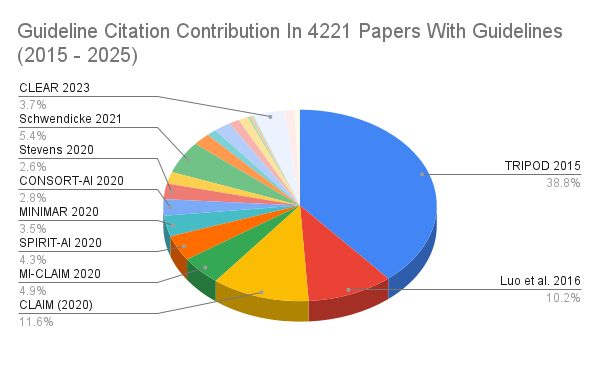
\includegraphics[width=0.8\textwidth]{Citation Contribution (2015 - 2025).png}
    \caption{CC (2015 - 2025)}
    \label{fig:cc2015}
\end{figure}

\begin{figure}[htbp]
    \centering
    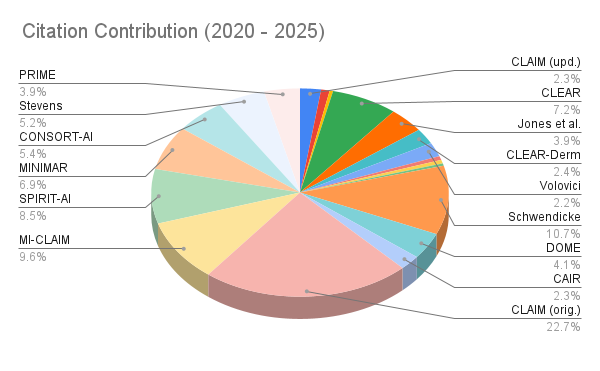
\includegraphics[width=0.8\textwidth]{Citation Contribution (2020 - 2025).png}
    \caption{CC (2020 - 2025)}
    \label{fig:cc2020}
\end{figure}


Citation patterns reveal that a small number of established frameworks dominate the majority of references. Specifically, TRIPOD (2015), Luo et al.(2016), and CLAIM (2020) together account for \~61\% of all non-review guideline citations. In contrast, more recently developed AI-specific standards–such as TRIPOD-AI (2024), CLAIM 2024, and FUTURE-AI (2025) –are cited in fewer than 5\% of papers that reference guidelines.

\newpage

\begin{table}[htbp]
\centering
\caption{Summary of AI in Medical Imaging and Guideline Citations (2015–2026, 2020–2026)}
\begin{tabular}{l r}
\hline
\textbf{Metric} & \textbf{Value} \\
\hline
Total AI in Medical Imaging Papers (2015–2026) & 36,187 \\
Review/Systematic Reviews (2015–2026) & 5,474 \\
Non-Reviews (2015–2026) & 30,713 \\
2015–2026 Guideline Citations & 4,221 \\
2015–2026 Guideline Citations (Non-Review) & 3,092 \\
Papers that used the guidelines (2015–2026) & 10.07\% \\
\hline
Total AI in Medical Imaging Papers (2020–2026) & 24,523 \\
Review/Systematic Reviews (2020–2026) & 4,652 \\
Non-Reviews (2020–2026) & 19,871 \\
2020–2026 Guideline Citations & 2,153 \\
2020–2026 Guideline Citations (Non-Review) & 1,355 \\
Papers that used the guidelines (2020–2026) & 6.82\% \\
\hline
\end{tabular}
\end{table}

\begin{figure}[htbp]
    \centering
    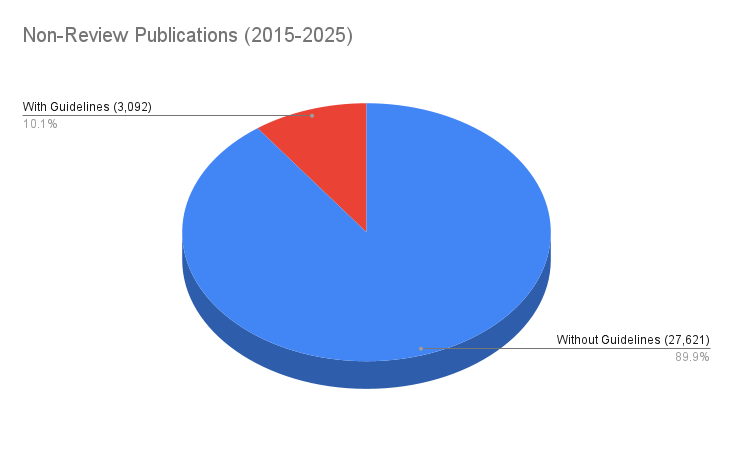
\includegraphics[width=0.8\textwidth]{Non-Review Publications (2015-2025).png}
    \caption{NRP (2015 - 2025)}
    \label{fig:nrp2015}
\end{figure}

\newpage

\begin{figure}[htbp]
    \centering
    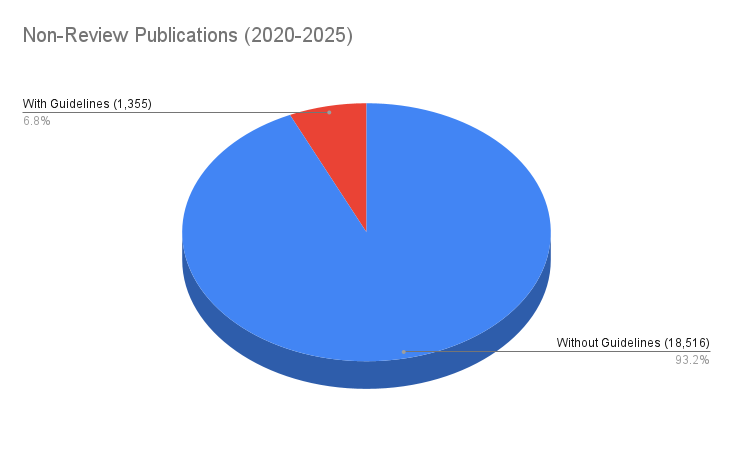
\includegraphics[width=0.8\textwidth]{Non-Review Publications (2020-2025).png}
    \caption{NRP (2020 - 2025)}
    \label{fig:nrp2020}
\end{figure}

This disparity of citations across guidelines indicates that the introduction of updated or new guidelines does not guarantee their adoption. Surveys conducted among UK-based medical imaging and radiotherapy (MIRT) professionals \cite{nikolaosstogiannos_2024_black} and various studies \cite{belue_2023_the,burakkoak_2025_adherence} identifies recurring barriers, including insufficient enforcement by journals and institutions, low levels of author/clinician awareness, the complexity of newer checklists, and the absence of regulations/protocols to facilitate compliance. Without more vigorous enforcement and more defined requirements, adoption of guidelines is likely to remain low,  which in turn weakens transparency, reproducibility, and trust in AI systems.

\section{Evaluation}

This review evaluated the state of AI adoption in medical imaging with a focus on adherence to standardized reporting guidelines such as CLAIM 2024, TRIPOD-AI, and FUTURE-AI. Fewer than 7\% of papers, excluding review and systematic reviews from 2020 to 2025, referenced these guidelines, even as updated frameworks became available. Older standards (e.g., TRIPOD 2015, CLAIM 2020) dominated citations, indicating hesitation in the uptake of more recent, AI-focused frameworks.

These trends can be observed in the independent evaluations of CLAIM adherence as well. A prostate MRI AI study (n = 53) found that several original CLAIM items were underreported in more than half of papers -- including de-identification methods (77\% missing), handling missing data (68\% missing), rationale for ground truth selection (47\% missing), and inclusion of failure analyses (92\% missing). Notably, models in the lowest compliance quartile (mean AUC = 0.78) performed significantly worse than those in the highest quartile (mean AUC = 0.89, p = 0.003) \cite{belue_2023_the}.

Similarly, an umbrella review of 26 reviews (874 studies) and 421 individual studies reported median CLAIM compliance rates of \~63-68\%, with at least 11 checklist items underreported in half or more of the studies. While compliance modestly improved after CLAIM’s introduction (p = 0.004), reliability analyses were rare (11\% of reviews), and item applicability was often inconsistent across study types \cite{burakkoak_2025_adherence}.

These findings further reinforce this review’s conclusion that reporting practices remain inconsistent, with low adherence undermining reproducibility, trust, and clinical applicability. Papers often demonstrated limited prospective validation, weak integration into clinical workflows, and inadequate attention to principles such as explainability, fairness, and robustness that establish trust.

The value of this review lies in combining quantitative citation analysis with qualitative literature synthesis to identify patterns in both technical and procedural aspects of AI development and adoption within the medical imaging domain. However, this study is subject to several limitations. First, citation data were collected exclusively from PubMed, except for one guideline. As a result, the findings may not apply to other databases such as Scopus, arXiv, IEEE publications, and others. Second, citations of a paper do not necessarily imply adherence to that paper, meaning that collected guideline uptake rates may be inflated. Third, the analysis focused exclusively on medical journals in English, potentially overlooking non-English publications and other applications of the guidelines.

\section{Discussion}
The findings highlight an ongoing gap between advances in AI capabilities for medical imaging and the adoption of practices necessary in establishing trust for clinical deployment. Low adherence to guidelines does not stem from their availability, but from systemic barriers such as limited awareness among researchers and clinicians, insufficient editorial and institutional enforcement, and the complexity of newer reporting standards.

Addressing these barriers requires a multifaceted approach. First, embedding explainability and trustworthiness principles into reporting requirements could ensure that model transparency, fairness, and robustness are evaluated alongside accuracy. Second, stronger enforcement mechanisms–whether through journal policies, institutional mandates, or funding requirements–are needed to improve compliance. Third, the development of tools such as automated compliance checkers, integrated authoring templates, or reviewer guidelines could further support adherence.

\section{Conclusion}
Advancements in artificial intelligence for medical imaging have achieved outstanding technical results in tasks like segmentation, detection, and classification. Despite the demonstrated high performance of these technologies, their implementation in clinical settings continues to be constrained by challenges related to trust and the absence of standardized reporting practices. This review revealed that fewer than 7\% of published studies reference or utilize established guidelines, despite the recent introduction of updated frameworks like CLAIM 2024, TRIPOD-AI, and FUTURE-AI. The low adoption rates in this study identify a path forward and reveal underlying systemic issues, including insufficient enforcement, limited awareness, and the complexities of these guidelines. Incorporating explainability and trust principles into reporting requirements, alongside enforcing guideline usage, is essential for supporting the transparency, reproducibility, and reliable integration of AI into clinical practice.

Further research on the adherence to guidelines should expand citation analyses to additional databases, regions, and non-English literature. Furthermore, empirical studies on whether guideline adherence improves deployment/clinical success would be helpful to assess the need for guidelines. In addition, qualitative interviews with authors, reviewers, and editors may help identify barriers and incentives for broader adoption.

\section{Acknowledgements}
The author acknowledges the use of generative AI tools for summarizing literature and assisting with drafting, structuring, and refining sections of this paper, as well as Grammarly for improving language clarity and consistency. Appreciation is also expressed to classmates for their constructive feedback,  to the teaching assistant for their support during the semester, and to the course instructor for their invaluable guidance and insights.

\bibliographystyle{splncs04}
\bibliography{sample}

\end{document}